\documentclass{article}
\usepackage{iclr2025_conference}
\usepackage{amsmath,amssymb}
\usepackage{amsthm}
\newtheorem{proposition}{Proposition}
\usepackage{graphicx}
\usepackage{booktabs}
\usepackage{xcolor}
\usepackage{natbib}
\usepackage[colorlinks=true,allcolors=blue]{hyperref}
\graphicspath{{figures/}}
\renewcommand{\topfraction}{0.95}
\renewcommand{\bottomfraction}{0.6}
\renewcommand{\textfraction}{0.05}
\renewcommand{\floatpagefraction}{0.9}
\setlength{\textfloatsep}{7pt plus 2pt minus 3pt}
\setlength{\intextsep}{8pt plus 2pt minus 2pt}
\setlength{\abovecaptionskip}{4pt}

\usepackage{xspace}
\newcommand{\PKPS}{PKPS\xspace}
\newcommand{\eps}{\varepsilon}

\title{Query Routing with Cached Responses}
\author{Anonymous}

\begin{document}
\maketitle

\begin{abstract}
An operator serving an expensive flagship model would often be willing to
answer some queries with a cheaper substitute, provided the substitute's
response is close to what the flagship would have said. We study this
problem in the setting that reflects deployed practice: the available
evidence is caches of raw model responses --- unlabeled, unscored, and with
no requirement that different models answered the same queries. We localize
the product-kernel perspective space (\PKPS) at each incoming query, which
yields a per-query behavioral geometry over models from unpaired caches;
the candidate nearest the flagship in this geometry is a good substitute,
matching routing with hidden task labels while using no metadata. To
offload \emph{safely} we attach a contract: a query is served by the
substitute only if the predicted deviation from the flagship is within a
tolerance $\eps$, calibrated so that
$P(\text{deviation} > \eps) \le \alpha$. The required confidence signal is
a kernel regression of realized same-query deviations, and we show both
empirically and by a variance argument that same-query pairs are necessary
for this component --- but that the small paired sample every calibrated
policy must already collect (candidate generations on a few hundred of the
operator's own queries; compute, not labels) is sufficient: it certifies a
median 90\% of traffic at $(\eps{=}0.5, \alpha{=}10\%)$ on a combined pool
of 138 models, within five points of full-pairing and near the oracle
ceiling. We measure the price of certification (a knee near $N \approx 800$
own-traffic queries, predictable in advance from query embeddings and a
small pilot), the validity of the gate, and the failure mode: traffic from
tasks absent from the cache silently exceeds the violation budget.
\end{abstract}

\section{Introduction}

Serving a frontier language model is expensive, and much of the traffic it
receives does not need it. Per-token prices across a deployed fleet
commonly span one to two orders of magnitude, so an operator who can
identify which queries a cheaper model would answer \emph{like the
flagship} can offload those queries and keep the rest, cutting the serving
bill with a bounded effect on what users see.

The evidence available for this decision is, in practice, caches of raw
responses: the flagship's own responses to logged traffic, and responses
of candidate models to whatever prompts they happen to have been run on
--- public benchmark dumps, prior evaluations, sampled traffic. These
caches are large but inconvenient. They carry no ground-truth labels or
judge scores (scoring is the expensive part of evaluation; generation is
not). Different models have answered different query sets, so the caches
are unpaired. And they carry no reliable task taxonomy. Most prior routing
work assumes at least one of these resources --- per-query quality labels,
task labels, or a paired evaluation matrix --- that this setting does not
provide.

Two problems must be solved with this evidence alone. First,
\emph{selection}: for each incoming query, which candidate would respond
most like the flagship? Second, \emph{certification}: for which queries can
we bound the risk of offloading --- serve the substitute only when
$P(\lVert x_{\text{sub}} - x_{\text{flag}}\rVert > \eps) \le \alpha$ for an
operator-chosen tolerance $\eps$ and budget $\alpha$? Selection turns out
to be the easy half. Certification requires a per-query error prediction
plus a calibration set, and it is here that the structure of the problem
--- what can and cannot be estimated from unpaired caches --- becomes
interesting.

We make four contributions. (1)~A router built from cached responses only:
a query-localized \PKPS geometry supplies the substitute (no labels, no
task metadata, no pairing), a kernel regression of realized same-query
deviations supplies the confidence, and a conformal cutoff supplies the
guarantee. (2)~Evidence that the label-free pick matches routing with
hidden task labels on a combined, unlabeled pool of two evaluation suites
(138 models), and an account of when selection is easy (target rank,
candidate count, cache density all act through a single quantity, the
neighbor-availability floor). (3)~An analysis of the confidence component:
its estimand decomposes so that everything except a same-query co-movement
term is estimable from unpaired caches, and that term resists both
plug-in and bias-corrected cross-query estimators for a variance reason
--- same-query differencing is the unique coupling that cancels the
per-query random effect sample-wise. The practical consequence is
positive: the paired sample that conformal calibration already requires,
reused as regression anchors, reaches within five points of the
full-pairing ceiling. (4)~An operational account: the certified volume as
a function of the paired-sample budget, with a knee predictable in advance
from query embeddings and a small pilot; the validity of the gate as a
function of calibration size; and a stated failure mode under task-level
distribution shift.

\section{Setting}

Let $f_1, \dots, f_n$ be models with cached responses. Model $f_i$ has
answered a query set $Q_i$; for $q_j \in Q_i$ we observe a response
embedding $x_{ij} \in \mathbb{R}^d$ and a query embedding
$u_j \in \mathbb{R}^{d_q}$. The query sets $Q_i$ may differ arbitrarily
across models, and no scores or task labels are observed. One model $f_*$
is the flagship being served; its responses to the operator's traffic
exist by definition. For an incoming query $q^*$ the router either serves
the flagship or picks a substitute $r(q^*)$ from a candidate pool and
serves it. The realized error of an offloaded query is the behavioral
deviation $\lVert x_{r,q^*} - x_{*,q^*} \rVert$; we do not assume
correctness scores exist, so behavioral fidelity is the objective rather
than a proxy.

The operator specifies a contract $(\eps, \alpha)$: among offloaded
queries, deviations above $\eps$ should have frequency at most $\alpha$.
Throughout, evaluation is leave-query-out: no model's response to an
evaluation query enters any geometry, regression, or calibration used to
route that query.

\section{The router}
\label{sec:method}

The router has three components: a pick, a confidence, and a gate.

\paragraph{Pick: the \PKPS geometry localized at $q^*$.}
The product-kernel perspective space compares models $i, i'$ through
\begin{equation}
A_{ii'} \;=\; \frac{\sum_{j \in Q_i} \sum_{l \in Q_{i'}}
  k_Q(u_j, u_l)\, k_R(x_{ij}, x_{i'l})}
 {\sum_{j \in Q_i} \sum_{l \in Q_{i'}} k_Q(u_j, u_l)},
\label{eq:pkps}
\end{equation}
which requires no shared queries. To route we localize this comparison at
the incoming query: each anchor's contribution is weighted by
$w_j = k_\sigma(u_j, u^*)$. Under a linear response kernel the localized
comparison factorizes into per-model statistics: model $i$ is represented
by the weighted mean of its own cache,
$\phi_i(q^*) = \sum_{j \in Q_i} w_j x_{ij} / \sum_{j \in Q_i} w_j$, and
the pick is the candidate minimizing
$\lVert \phi_i(q^*) - \phi_*(q^*) \rVert$. Because $\phi_i$ uses only
model $i$'s own rows, merging heterogeneous caches cannot contaminate the
geometry, and fully disjoint query sets are handled without modification.
The bandwidth $\sigma$ is set to a fixed fraction of the median
anchor-query distance; a leak-free cross-validation on anchors selects
the same value (Appendix).

\paragraph{Confidence: deviation regression on the calibration sample.}
The gate needs, for each query, a prediction of the deviation the pick
would realize. The estimand is a localized same-query expectation, and it
decomposes as
\begin{equation}
\mathbb{E}\,\lVert x_{i,q} - x_{*,q} \rVert^2
 = \lVert \mu_i - \mu_* \rVert^2 + \operatorname{tr}\Sigma_i
 + \operatorname{tr}\Sigma_* - 2\operatorname{tr}\operatorname{Cov}(x_i, x_*),
\label{eq:decomp}
\end{equation}
with means, variances, and the covariance taken over queries near $q^*$.
The first three terms are per-model and therefore estimable from unpaired
caches --- they are the \PKPS quantities. The co-movement term is a joint
moment: responses to the same query share a large query-driven component
(models echo the prompt), and this component cancels only in same-query
differences. Section~\ref{sec:why} shows that estimators built without
same-query pairs fail here, for variance rather than identifiability
reasons. The confidence we use is the direct kernel regression of realized
deviations on same-query pairs,
\begin{equation}
\widehat{D}_i(q^*) \;=\;
\frac{\sum_{j \in P_i} w_j\, \lVert x_{ij} - x_{*j} \rVert}
     {\sum_{j \in P_i} w_j},
\label{eq:pdcal}
\end{equation}
where $P_i$ is the set of queries answered by both $f_i$ and the flagship
in a designated anchor sample. Crucially, this sample need not come from
the caches: the flagship's responses to the operator's traffic exist, and
running each candidate once over a few hundred logged queries is a
generation cost, not a labeling cost. The same sample is required by any
calibrated policy (below), so the confidence adds no assumption beyond
what the guarantee itself already demands.

\paragraph{Gate: conformal cutoff.}
The operator's own paired sample is split in half: one half provides the
regression anchors $P_i$ in \eqref{eq:pdcal}, the other calibrates the
gate. On the calibration half we observe (confidence, realized deviation)
pairs; the gate offloads a query when its confidence falls below the
largest cutoff whose empirical calibration violation
$P(\text{dev} > \eps \mid \text{offloaded})$ is at most $\alpha$. Any
policy that promises a deviation bound must observe realized deviations to
calibrate it, and a realized deviation is by definition the flagship and a
candidate answering the same query --- so this paired sample is the
irreducible cost of the guarantee, for every method.

\section{Experiments}
\label{sec:experiments}

\paragraph{Data.} We use two evaluation suites with Gemini-embedded
queries and responses: a fully paired core of 93 models on 1{,}529 queries
over 18 tasks, and an unpaired suite of 45 models on 6{,}808 queries over
16 tasks with roughly 10\% incidental overlap. Their union is treated as
one unlabeled pool: 138 models, 8{,}457 queries, 34 hidden tasks; task and
suite labels are hidden from all routers and used only to define reference
baselines. The flagship is the pool's best model by anchor mean score
(per suite); candidate pools are either unrestricted or restricted to
models of at most 13B parameters (a serving-cost proxy).

\paragraph{Protocol.} Unless noted, results use one protocol: 400
evaluation queries, 400 regression-anchor queries, and 400 gate-calibration
queries per seed, disjoint, all excluded from every geometry; 15 seeds.
Certified volumes are reported as median [IQR] across seeds because the
gate's outcome is bimodal: it either certifies its typical volume or, when
the calibration draw cannot support the contract, abstains entirely ---
volume zero with the contract intact. Abstention rates are reported
alongside. Violations are reported over certifying seeds.

\begin{figure}[t]
\centering
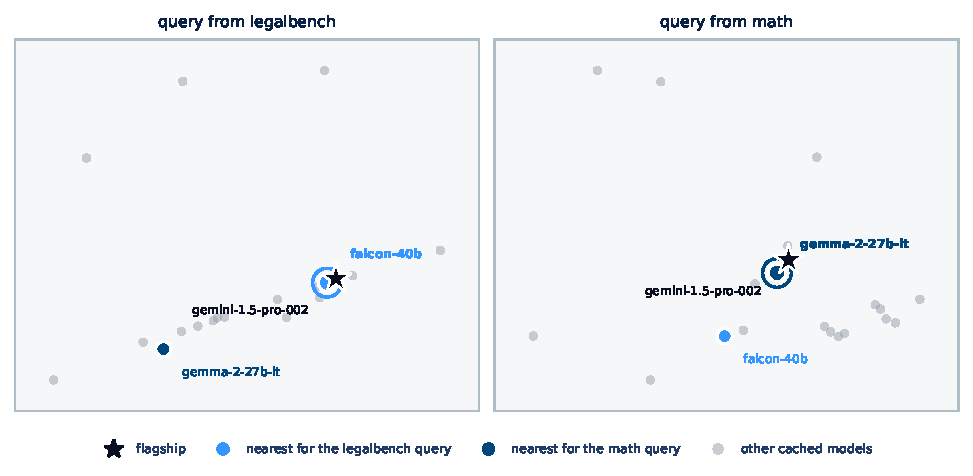
\includegraphics[width=\linewidth]{fig1_concept}
\caption{One response cache, two queries. The same cached models, embedded
by the \PKPS geometry localized at a LegalBench query (left) and a MATH
query (right); the flagship is starred and both queries' nearest
candidates are highlighted in both panels. The substitute nearest the
flagship changes with the query; positions are 2-D projections constrained
to preserve the nearest-candidate relation.}
\label{fig:concept}
\end{figure}

\subsection{The pick, and the guarantee it supports}

Figure~\ref{fig:payoff}a evaluates selection alone on the combined pool:
route each evaluation query to the candidate nearest the flagship, measure
the realized deviation of the pick. The label-free \PKPS pick attains mean
deviation 0.378, statistically indistinguishable from routing with the
hidden task labels (0.384) and well ahead of the static (non-localized)
geometry (0.421) and random (0.548); the hindsight-best pick achieves
0.183. Selection difficulty is governed by a single quantity, the
neighbor-availability floor --- the deviation of the hindsight-best
candidate: the floor and the \PKPS error trace the same curve as the
target's rank varies, as the candidate pool grows, and as the cache
densifies (Appendix).

Figure~\ref{fig:payoff}b is the paper's central result. At budget
$\alpha = 10\%$ the router sweeps the tolerance $\eps$ and certifies, at
each point, the median fraction of traffic it can offload with
$P(\text{dev} > \eps) \le \alpha$. At $\eps = 0.5$ it certifies a median
90\% of traffic on the unrestricted pool (abstaining in 3 of 15 seeds) and
24\% on the $\le$13B pool; the oracle --- the same gate given the realized
deviations --- certifies 93\%. Score-free baselines do not appear on this
plot because they cannot: a leaderboard pick, the static geometry, and
random selection have no per-query error signal, so their violation rate
at a given $\eps$ is a fixed population property (38--63\% at
$\eps = 0.3$; Table~\ref{tab:baselines}) that no volume choice can lower.
The per-query contract requires a per-query error predictor.
Figure~\ref{fig:payoff}c converts certified volume to money: at a 25$\times$
flagship-to-substitute price ratio, offloading to $\le$13B substitutes
saves roughly a quarter of the flagship bill at $\eps = 0.5$ and up to
three quarters at looser tolerances.

\begin{figure}[t]
\centering
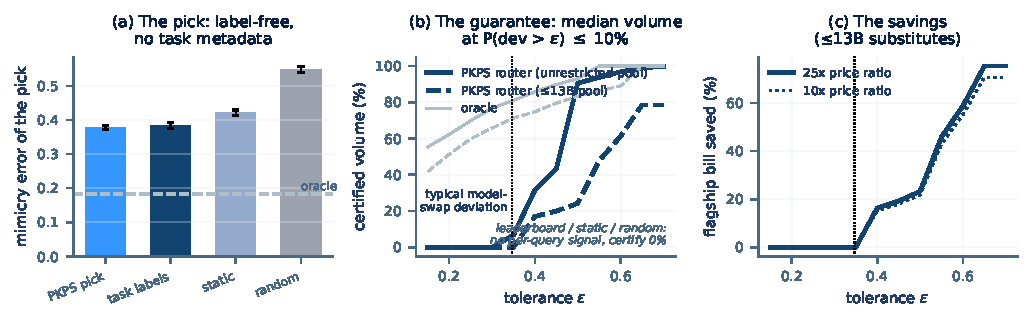
\includegraphics[width=\linewidth]{fig2_payoff}
\caption{Does it pay? (a)~Selection on the combined unlabeled pool:
the label-free \PKPS pick matches routing with hidden task labels;
dashed line is the hindsight-best floor. (b)~Certified volume at
$P(\text{dev} > \eps) \le 10\%$, median over 15 seeds; the oracle gates
the same picks with realized deviations. Methods without a per-query
error signal certify zero volume at any tolerance
(Table~\ref{tab:baselines}). (c)~Flagship bill saved on the $\le$13B pool
at two price ratios.}
\label{fig:payoff}
\end{figure}

\subsection{Why the confidence needs exact pairs, and why that is cheap}
\label{sec:why}

Figure~\ref{fig:why}a compares confidence signals under the single
protocol above, holding the pick and gate fixed. The best fully unpaired
confidence --- the localized mean distance, i.e.\ the pick's own geometry
--- certifies a median 41\% with an interquartile range reaching zero
(abstaining in 40\% of seeds). The deviation regression anchored on the
operator's paired sample certifies 90\%; anchoring it instead on all
shared queries in the suites (full pairing, roughly 1{,}400 shared anchors
per pair against the flagship) certifies 95\%. The oracle line is 93\%.
The gap that matters is the first one: means-only confidence is
qualitatively insufficient, and the decomposition \eqref{eq:decomp} says
why --- it omits both variance terms and the co-movement term, and the
latter is the dominant contributor because responses echo their prompts.

Two natural attempts to recover the co-movement term without pairs fail,
and the failure is informative. The plug-in bound that sets
$\operatorname{Cov} = 0$ certifies approximately zero: the omitted term is
most of the variance, not a correction. A soft-coupled estimator that
differences responses to \emph{similar} queries, with the query-difference
penalty explicitly removed using within-model distance curves (an unbiased
correction under an additive query effect), drowns: it subtracts two
nuisance-dominated quantities to extract a small signal, and its ordering
degrades below chance. The general statement is a variance argument.
The query effect $g(q)$ is a per-query random effect that dominates
response variation; same-query differencing is the unique coupling that
cancels it sample-wise rather than in expectation, so every cross-query
estimator carries variance at least the $g$-variability at the closest
available query match. Benchmark caches contain no near-duplicate queries,
so that variance exceeds the model-difference signal. This is the
matched-pairs design argument: matching removes the subject effect, and
these data contain no twins. Figure~\ref{fig:why}b shows the controlled
version: with per-model cache size fixed, the paired regression's
certified volume falls as flagship--candidate anchor overlap drops from
100\% to 50\% and is undefined at 0\%, while the soft-coupled estimator
earns exactly its exact-match content and nothing more.

The positive consequence: because certification already forces the
operator to collect realized deviations --- candidate generations on a few
hundred of their own queries --- the necessary pairing is already in hand.
Equation~\eqref{eq:pdcal} anchored on that sample is within five points of
the full-pairing ceiling, and on-traffic anchors are worth several times
their count in suite-wide anchors (Appendix).

\begin{figure}[t]
\centering
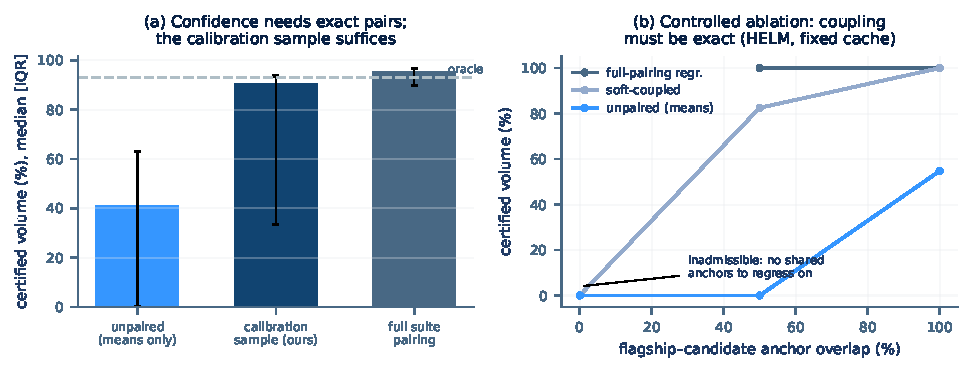
\includegraphics[width=0.9\linewidth]{fig3_why}
\caption{Why it works. (a)~Certified volume by confidence signal under one
protocol (median [IQR], 15 seeds): unpaired means are qualitatively
insufficient; the deviation regression \eqref{eq:pdcal} anchored on the
operator's calibration sample reaches within five points of full-suite
pairing and the oracle line. (b)~Controlled pairing ablation (paired
suite, fixed 50\% cache per model): the regression requires shared
anchors --- inadmissible at zero overlap --- and soft coupling over
similar queries earns only its exact-match content, consistent with the
variance argument in \S\ref{sec:why}.}
\label{fig:why}
\end{figure}

\subsection{Cost, validity, and limits}

Figure~\ref{fig:ops}a prices the paired sample. Sweeping the total budget
$N$ (half regression anchors, half gate calibration, nested within seed so
the comparison is paired), certified volume on the unrestricted pool
reaches its plateau near $N \approx 800$ own-traffic queries; below
$N \approx 300$ the gate itself is unreliable and outcomes are bimodal.
The knee is predictable before collecting anything: the confidence's
signal-to-noise crosses one at
$N^* = s^2 / (\kappa \tau^2)$, where the kernel coverage $\kappa$ is
computable from query embeddings alone and the noise and signal scales
$s^2, \tau^2$ from a pilot of roughly one hundred pairs; on these data
$N^* \approx 217$ anchors, matching the observed knee within a factor of
two, with the calibration side adding a few hundred more.

Figure~\ref{fig:ops}b examines the gate rule. The empirical cutoff tracks
the budget from above as calibration grows (violations 8--10\% at
volumes near 90\%); a Clopper--Pearson cutoff is safe at every size but
abstains in most seeds at these calibration sizes --- a provable gate
needs either more calibration data or a weaker correction.
Figure~\ref{fig:ops}c states the failure mode. When evaluation traffic
comes from tasks entirely absent from the cache, the confidence
distribution barely shifts (AUC 0.62 for detecting novelty --- too weak to
gate on), the gate offloads novel-task queries at a normal rate, and the
achieved violation exceeds the budget (12.6\% against 10\% on the
unrestricted pool). The guarantee is therefore conditional on traffic
exchangeability with the calibration sample; detecting out-of-cache
queries is an open problem, and the natural coverage statistics
(effective local sample size) are anti-correlated with novelty on these
data.

\begin{figure}[t]
\centering
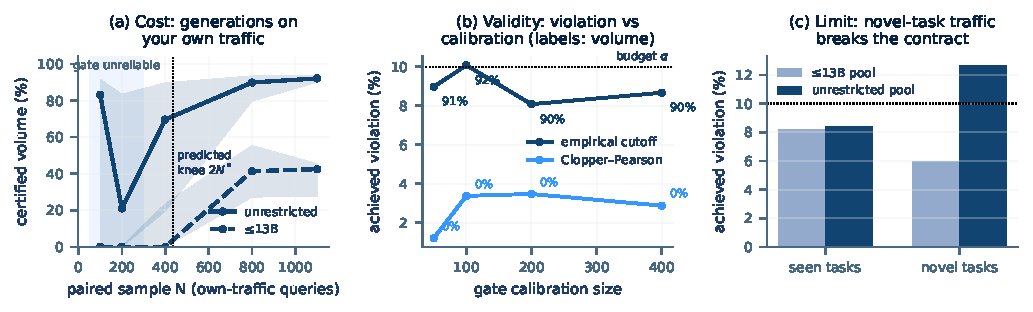
\includegraphics[width=\linewidth]{fig4_ops}
\caption{Cost and limits. (a)~Certified volume vs.\ the paired-sample
budget $N$ (median [IQR], nested subsets, 10 seeds); the region below
$N \approx 300$ is shaded because the gate itself is unreliable there;
dotted line marks the predicted knee $2N^*$. (b)~Achieved violation vs.\
gate-calibration size for the empirical and Clopper--Pearson cutoff rules
(labels: median certified volume; the conservative rule mostly abstains).
(c)~Traffic from tasks absent from the cache exceeds the violation budget
on the unrestricted pool; the guarantee is conditional on
exchangeability.}
\label{fig:ops}
\end{figure}

\begin{table}[t]
\centering
\caption{The confidence ladder under one protocol (combined pool,
unrestricted candidates, $(\eps{=}0.5, \alpha{=}10\%)$, 15 seeds).
Volumes are medians; violations are over certifying seeds.}
\label{tab:ladder}
\small
\begin{tabular}{lllrrr}
\toprule
confidence & coupling & pairing assumed & volume & abstain & viol.\\
\midrule
localized means & none (unpaired) & none & 41\% & 40\% & .11\\
deviation regr.\ (ours) & exact & calibration sample only & 90\% & 20\% & .11\\
deviation regr.\ (full) & exact & all shared suite queries & 95\% & 0\% & .09\\
oracle & --- & (peeks at eval) & 93\% & 0\% & .11\\
\bottomrule
\end{tabular}
\end{table}

\begin{table}[t]
\centering
\caption{Methods without a per-query error signal cannot hold a contract:
their violation rate at tolerance $\eps$ is a fixed population property,
independent of how much traffic is offloaded (combined pool, eval split).}
\label{tab:baselines}
\small
\begin{tabular}{lcccccc}
\toprule
 & \multicolumn{3}{c}{$\le$13B pool} & \multicolumn{3}{c}{unrestricted}\\
$\eps$ & 0.1 & 0.3 & 0.5 & 0.1 & 0.3 & 0.5\\
\midrule
leaderboard pick & 70\% & 46\% & 28\% & 63\% & 38\% & 19\%\\
random pick      & 77\% & 56\% & 39\% & 71\% & 48\% & 32\%\\
\bottomrule
\end{tabular}
\end{table}

\section{Discussion}

The two halves of the router obey different laws. The pick --- a first
moment of the localized product kernel --- factorizes over models, needs
no pairing of any kind, and is robust to merging arbitrary caches; this is
the regime where the \PKPS construction, comparing responses to similar
rather than identical queries, does exactly what it was designed to do.
The guarantee --- a second moment --- does not factorize: predicting a
same-query difference requires observing same-query differences, for
variance rather than identifiability reasons. What makes the method
practical is that the requirement collapses onto a sample the guarantee
already charges for. We read this as a general design principle for
routing systems built on cached responses: spend the generation budget on
your own traffic, not on more benchmark coverage --- on-traffic anchors
were worth several times their count in suite anchors throughout our
experiments.

Three limitations are explicit in the results. The contract is conditional
on traffic exchangeability, and novel-task traffic breaks it silently;
until an out-of-cache detector exists, the guarantee should be stated for
in-distribution traffic. The empirical gate rides the budget from above
and occasionally abstains; a provably valid gate at these calibration
sizes remains open. And the behavioral objective bounds deviation in an
embedding space; where correctness labels exist, deviation is a proxy
whose adequacy should be checked (on our suites, behavioral policies held
95--99\% of flagship score at conservative budgets; Appendix).

\end{document}
